% java BurrowsWheeler - < inputs\dickens.txt | java MoveToFront - | java Huffman - > inputs\dickens_compressed.txt
% du -b dickens.txt | awk '{ print $1, "* 8" }' | bc
% Use this template to write your solutions to COS 423 problem sets

\documentclass[12pt]{article}
\usepackage[utf8]{inputenc}
\usepackage{amsmath, amsfonts, amsthm, amssymb, algorithm, graphicx, mathtools, xfrac}
\usepackage[noend]{algpseudocode}
\usepackage{fancyhdr, lastpage}
\usepackage{booktabs}
\usepackage{multirow}
\usepackage{graphicx}
\usepackage{pgfplots}
\usepackage[vmargin=1.20in,hmargin=1.25in,centering,letterpaper]{geometry}
\setlength{\headsep}{.50in}
\setlength{\headheight}{15pt}

% Landau notation
\DeclareMathOperator{\BigOm}{\mathcal{O}}
\newcommand{\BigOh}[1]{\BigOm\left({#1}\right)}
\DeclareMathOperator{\BigTm}{\Theta}
\newcommand{\BigTheta}[1]{\BigTm\left({#1}\right)}
\DeclareMathOperator{\BigWm}{\Omega}
\newcommand{\BigOmega}[1]{\BigWm\left({#1}\right)}
\DeclareMathOperator{\LittleOm}{\mathrm{o}}
\newcommand{\LittleOh}[1]{\LittleOm\left({#1}\right)}
\DeclareMathOperator{\LittleWm}{\omega}
\newcommand{\LittleOmega}[1]{\LittleWm\left({#1}\right)}

% argmin and argmax
\newcommand{\argmin}{\operatornamewithlimits{argmin}}
\newcommand{\argmax}{\operatornamewithlimits{argmax}}

\newcommand{\calP}{\mathcal{P}}
\newcommand{\Z}{\mathbb{Z}}
\newcommand{\R}{\mathbb{R}}
\newcommand{\Exp}{\mathbb{E}}
\newcommand{\Q}{\mathbb{Q}}
\newcommand{\sign}{\mathrm{sign\ }}
\newcommand{\abs}{\mathrm{abs\ }}
\newcommand{\eps}{\varepsilon}
\newcommand{\zo}{\{0, 1\}}
\newcommand{\SAT}{\mathit{SAT}}
\renewcommand{\P}{\mathbf{P}}
\newcommand{\NP}{\mathbf{NP}}
\newcommand{\coNP}{\co{NP}}
\newcommand{\co}[1]{\mathbf{co#1}}
\renewcommand{\Pr}{\mathop{\mathrm{Pr}}}

% theorems, lemmas, invariants, etc.
\newtheorem{theorem}{Theorem}
\newtheorem{lemma}[theorem]{Lemma}
\newtheorem{invariant}[theorem]{Invariant}
\newtheorem{corollary}[theorem]{Corollary}
\newtheorem{definition}[theorem]{Definition}
\newtheorem{property}[theorem]{Property}
\newtheorem{proposition}[theorem]{Proposition}

% piecewise functions
\newenvironment{piecewise}{\left \{\begin{array}{l@{,\ }l}}
{\end{array}\right.}

% paired delimiters
\DeclarePairedDelimiter{\ceil}{\lceil}{\rceil}
\DeclarePairedDelimiter{\floor}{\lfloor}{\rfloor}
\DeclarePairedDelimiter{\len}{|}{|}
\DeclarePairedDelimiter{\set}{\{}{\}}

\makeatletter
\@addtoreset{equation}{section}
\makeatother
\renewcommand{\theequation}{\arabic{section}.\arabic{equation}}

% algorithms
\algnewcommand\algorithmicinput{\textbf{INPUT:}}
\algnewcommand\INPUT{\item[\algorithmicinput]}
\algnewcommand\algorithmicoutput{\textbf{OUTPUT:}}
\algnewcommand\OUTPUT{\item[\algorithmicoutput]}


% Formating Macros

\pagestyle{fancy}
\lhead{\sc \hmwkClass\ $\; \;\cdot \; \;$ \hmwkSemester\ $\; \;\cdot \; \;$
Problem \hmwkAssignmentNum.\hmwkProblemNum}
%\chead{\sc Problem \hmwkAssignmentNum.\hmwkProblemNum}
%\chead{}
\rhead{\em \hmwkAuthorName\ $($\hmwkAuthorID$)$\/}
\cfoot{}
\lfoot{}
\rfoot{\sc Page\ \thepage\ of\ \protect\pageref{LastPage}}
\renewcommand\headrulewidth{0.4pt}
\renewcommand\footrulewidth{0.4pt}

\fancypagestyle{fancycollab}
{
    \lfoot{\textit{Collaborators: \hmwkCollaborators}}
}

\fancypagestyle{problemstatement}
{
    \rhead{}
    \lfoot{}
}

%%%%%% Begin document with header and title %%%%%%%%%%%%%%%%%%%%%%%%%

\begin{document}

%%%%%% Header Information %%%%%%%%%%%%%%%%%%%%%%%%%%%%%%%%%%%%%%%%%%%

%%% Shouldn't need to change these
\newcommand{\hmwkClass}{COS 255}
\newcommand{\hmwkSemester}{Spring 2016}

%%% Your name, in standard First Last format
\newcommand{\hmwkAuthorName}{Lukas Leung}
%%% Your NetID
\newcommand{\hmwkAuthorID}{lleung}

%%% The problem set number (just the number)
\newcommand{\hmwkAssignmentNum}{3}

%%% The problem number (just the number)
\newcommand{\hmwkProblemNum}{0}

%%% A list of your collaborators' NetIDs, separated by ", ".
%%% You can use a new line ("\\") in the middle to prevent a long
%%% list from overflowing.
\newcommand{\hmwkCollaborators}{}
%%% Sets the collaborator list to appear on the first page
\thispagestyle{fancycollab}

%%%%%%% begin Solution %%%%%%%%%%%%%%%%%%%%%%%%%%%%%%%%%%%%%%%%%%%%


%%%%%%% begin GrapeVine Problem %%%%%%%%%%%%%%%%%%%%%%%%%%%%%%%%%%%

\section{UVA Problem 12192: Grapevine}
~\indent In Quadradonia, all rural properties are square, all have the same area, all are perfectly flat and all
have the sides aligned to the North-South and West-East axes.
Since properties are flat, the hills in Quadradonia look like a series of huge stairs’ steps, with different
heights. In a certain mountain, an interesting situation occurs in a rectangular area of N ×M properties.
Starting from anywhere within the region, traversing it in the West to East direction, the properties
have non-descending heights. Similarly, traversing that region in the North to South direction, starting
from anywhere, the properties have also non-descending heights. \\
\indent A large wine company in Quadradonia wants to rent some properties from that region to grow wine
grapes. The company is interested in some special varieties of wine grapes, which are productive only
if grown in properties whose heights are within a certain interval. That is, the company is interested in
renting properties whose heights are equal to or higher than a given altitude L, and equal to or lower
than a given altitude U . To make it easier for harvesting, the rented properties must form a contiguous
area. And since everyone in Quadradonia likes squares, the area to be rented must have the shape of
a square. \\
\indent The company has not yet decided which variety of grapes it will grow, and therefore it has a list
of queries involving intervals, one for each grape variety. The figure below shows an area of interest
of dimensions 4 × 5 (in number of properties) with examples of areas the company could rent to grow
grapes in heights within the intervals given in the picture.

\begin{figure}[H]
    \centering
    \begin{tikzpicture}
        \draw[line width = 2, fill=white!80!black] (1, 0) rectangle (4, 3);
        \draw[step = 1, color = black, thick] (0, 0) grid (5, 4);

        \node at (0.5, 0.5) {23};
        \node at (0.5, 1.5) {16};
        \node at (0.5, 2.5) {16};
        \node at (0.5, 3.5) {13};

        \node at (1.5, 0.5) {51};
        \node at (1.5, 1.5) {33};
        \node at (1.5, 2.5) {21};
        \node at (1.5, 3.5) {21};

        \node at (2.5, 0.5) {66};
        \node at (2.5, 1.5) {33};
        \node at (2.5, 2.5) {33};
        \node at (2.5, 3.5) {25};

        \node at (3.5, 0.5) {83};
        \node at (3.5, 1.5) {45};
        \node at (3.5, 2.5) {35};
        \node at (3.5, 3.5) {33};

        \node at (4.5, 0.5) {93};
        \node at (4.5, 1.5) {50};
        \node at (4.5, 2.5) {35};
        \node at (4.5, 3.5) {34};
    \end{tikzpicture}
\end{figure}

\indent You must write a program that, given the description of the rectangular area of interest in the
mountain, and a list of queries containing height intervals, determines, for each query, the largest side,
in number of properties, of a contiguous square area with heights within the specified interval.

%%%%%%% end Problem %%%%%%%%%%%%%%%%%%%%%%%%%%%%%%%%%%%%%%%%%%%%%%%

\newpage

%%%%%%% Mathematical Formulation %%%%%%%%%%%%%%%%%%%%%%%%%%%%%%%%%%
\subsection{Mathematical Formulation}
Given an N x M board, where each $n_i$ < $n_{i+1}$ and $m_j$ < $m_{j+1}$ so that the smallest value is
in index (0, 0) and the largest is in (1, 1). We will determine the maximum square area that is within
the user specified bounds (L, U).

%%%%%%% Algorithm %%%%%%%%%%%%%%%%%%%%%%%%%%%%%%%%%%%%%%%%%%%%%%%%%

\subsection{Solution}

In our main functionality we will be reading in the data and storing it in a 1-D representation of a
2-D topological map. Each index will represent a square lot in this \textbf{int[N*M]}, int array of
size N*M. We use regular int values to store the Lower and Upper bounds (L,U) and number of cases (Q).
For each case, we will go through each row executing a \textbf{modified binary search} to search for
the index of the lot which is the lowest of the in-bound lots (left-most lowerbound). This is explained
in Algorithm II. Once this value is retrieved we use the fact that each $n_i$ < $n_{i+1}$ and $m_j$ < $m_{j+1}$
meaning that we \textbf{only need to check the diagonal} from this lowerBound to ensure that this square
is a valid one. We will record the maximum size and continue checking. We will terminate either on the
last row or the last possible row. i.e. if we have found 3 to be the max size, once we reach the second
to last row, we cannot find a better than 3 square so we are done.

\begin{algorithm}[H]
\caption{GrapeVine main}
\begin{algorithmic}
    \Procedure{main}{ }
        \State $reader \gets$ BufferedReader
        \State $stringBuilder \gets$ StringBuilder
        \State $line \gets$ reader.\Call{readLine}{ }
        \While{there is a new line}
            // get the dimentions of the board
            \State $N, M \gets$  line.\Call{split}{bySpace}
            \State Ensure N, M are in bounds
            \State $map \gets$ int[N][M] // this is actually 1-Dimensional
            \For{$i \in length(N)$}
                \State $splitLine \gets$ reader.\Call{readLine}{ }.\Call{splitLine}{bySpace}
                \For{$j \in length(M)$}
                    \State $map[i][j] \gets$ Integer.\Call{parseInt}{splitLine[j]}
                \EndFor
            \EndFor
            \State $Q \gets$ Integer.\Call{parseInt}{reader.readLine()}
            \State $stringBuilder \gets$ new StringBuilder()
            \While{$Q \neq 0$}
                \State $L, U \gets$ Lower and Upper bounds
                \State $max \gets$ 0
                \For{$i \in N$ \&\& $(N - i + 1) \textgreater max$}
                    \State $lowerIndex \gets$ lowerBound(map, i, (M-1), L) // see below
                    \If{lowerIndex == 0}
                        \State continue
                    \EndIf
                    \For{$j=max .. \textless M$}
                        \State $n \gets$ i + j
                        \State $m \gets$ lowerBound + j
                        \If{$n \ge N\ ||\ m \ge M\ ||\ map[n][m] \textgreater U$}
                            \State break
                        \EndIf
                        \If{$j+1 \textgreater max$}
                            \State $max \gets$ j + 1
                        \EndIf
                    \EndFor
                \EndFor
                \State stringBuilder.\Call{append}{max}
                \State Q--
            \EndWhile
            \State stringBuilder.\Call{append}{-}
            \State $line \gets$ reader.\Call{readLine}{ }
        \EndWhile
    \EndProcedure
\end{algorithmic}
\end{algorithm}

\newpage

The point of the following algorithm is to binary search a row within
the map and returns the lowest possible valid lot.

\begin{algorithm}[H]
\caption{GrapeVine get lower bound}
\begin{algorithmic}
    \Procedure{lowerBound}{int[] map, int row, int size, int L}
        \State $lower \gets$ 0, $higher \gets$ size, $answer \gets$ -1, mid
        \While{$lower \leq higher$}
            \State $mid \gets$ lower + (higher - lower) / 2
            \If{$map[row][mid] \geq L$}
                \State $answer \gets$ mid
                \State $higher \gets$ mid - 1
            \Else
                \State $lower \gets$ mid + 1
            \EndIf
        \EndWhile
    \EndProcedure
\end{algorithmic}
\end{algorithm}

%%%%%%% Correctness %%%%%%%%%%%%%%%%%%%%%%%%%%%%%%%%%%%%%%%%%%%%%%%

\subsection{Correctness}
%%%%%%% PROPOSITION 1 %%%%%%%%%%%%%%%
\begin{proposition}
~ \\ \indent The $lowerBound$ method will give us the index $m_j$ of the lot which has the lowest elevation within the bounds (U, L)
within the specified row $n_i$.
\end{proposition}

\begin{proof}
~ \\ \indent We begin this by stating that the length of any given row is $k+1$ and, since this method call is independent between
rows we can say that we are only looking at the elements $m_0, m_1, ..., m_k$ in row $n_i$. We do a binary search then,
our checking statement will be to see if the midpoint is within the bounds (U,L) s.t. first time through we check
$m_{k/2} \in (U,L)$. If in bounds, our new upper bound will be $m_{k/2-1}$, otherwise our new lower bound will be
$m_{k/2-1}$. This process is done until we have gone through the complete search (lg(k)).
\end{proof}

%%%%%%% PROPOSITION 2 %%%%%%%%%%%%%%%
\begin{proposition}
~ \\ \indent In any square area, the top left corner lot will have the lowest elevation and the bottom right will have
the largest area.
\end{proposition}

\begin{proof}
~ \\ \indent This is more or less given in the problem description but to put it into a mathematical formulation we say that given
the square area
\begin{center}$
\begin{bmatrix}
    x_{i,j}          & x_{(i+1),(j+1)} & \dots  & x_{(i),(j+k)}     \\
    x_{(i+1),j}      & x_{(i+1),(j+1)} & \dots  & x_{(i+1),(j+k)}   \\
    \vdots           & \vdots          & \ddots & \vdots            \\
    x_{(i+k),(j)}    & x_{(i+k),(j+1)} & \dots  & x_{(i+k),(j+k)}
\end{bmatrix}
$\end{center}
we are gauranteed that (1) $x_{i,j} \textless x_{i,(j+1)} \textless ... \textless x_{i,(j+k)}$
and (2) $x_{i,j} \textless x_{(i+1),j} \textless ... \textless x_{(i+k),j}$.  This translates
accross rows so that in (1) if we replace $i$ with $(i+1)...(i+k)$ the same relationship will hold
and similarly, replacing $j$ with $(j+1)...(j+k)$ in (2) will also hold.
\begin{center}$\therefore$ The lowest value will be $x_{i,j}$ and the highest will be $x_{(i+k),(j+k)}$.\end{center}
\end{proof}

%%%%%%% PROPOSITION 3 %%%%%%%%%%%%%%%
\begin{proposition}
~ \\ \indent Given the left most valid lot $x_{i,j}$ on a given row $i$, when we diagonally search through the topological map
we will find the maximum size square possible originating from that row (not unique). i.e. look at $x_{(i+1),(j+1)}
,x_{(i+2),(j+2)},...,x_{(i+p),(j+p)}$ where $0 \leq p \leq k = min(N,M)$.
\end{proposition}

\begin{proof}
~ \\ \indent Given $x_{i,j}$, we know from proposition 2 that $x_{i,j} \textless x_{i,(j+1)},\ x_{i,j}
\textless x_{(i+1),j}$, and \\ all three $\textless\ x_{(i+1),(j+1)} \implies$ as we go diagonally we are increasing
in area covered s.t. the bottom right corner, $x_{(i+p),(j+p)}$ for $i \le p \le k$ is the biggest and $x_{i,j}$ is
the smallest.Therefore the square matrix produced by this area is within the bounds (L,U) if both $x_{i,j}
\ and\ x_{(i+p),(j+p)} \in (L,U)$. Lets say the diagonal check will return that the $x_{(i+(p+1)),(j+(p+1))}$ fails
$\implies$ that all lots $x_{(i+(p+2)),(j+(p+1))},x_{(i+(p+3)),(j+(p+1))}$, ... ,$x_{(i+(p+k),(j+(p+1))}$ and
$x_{(i+(p+1)),(j+(p+2))}, x_{(i+(p+1)),(j+(p+3))},...,x_{(i+(p+1)),(j+(p+k))}$ will fail as well as all
$x_{(i+y),(j+z)}$ are also invalid $\forall\ (p+1)\ \textless\ y,z \leq\ k$ where $k \in min(N,M)$. This means that
all lots in the matrix below will be invalid.
\begin{center}
$
\begin{bmatrix}
    x_{(i+(p+1)),(j+(p+1))} & x_{(i+(p+1)),(j+(p+2))} & \dots  & x_{(i+(p+1)),(j+(p+k))} \\
    x_{(i+(p+2)),(j+(p+1))} & x_{(i+(p+2)),(j+(p+2))} & \dots  & x_{(i+(p+2)),(j+(p+k))} \\
    \vdots                  & \vdots                  & \ddots & \vdots                  \\
    x_{(i+(p+k)),(j+(p+1))} & x_{(i+(p+k)),(j+(p+2))} & \dots  & x_{(i+(p+k)),(j+(p+k))}
\end{bmatrix}
$
\end{center}
Assume the valid lot matrix starting at $x_{i,(j+1)}$ as its top left corner is larger than the lot matrix we have just
found. $\implies$ this lot must contain at least $x_{(i+(p+1)),(j+(p+2))}$ which would make the matrix size
(p+1), one bigger than the lots previously found. However we just showed that $x_{(i+(p+1)),(j+(p+2))}$ which is a
contradiction. we can replace this with any $x_{i,(j+m)})$ where $1 \leq m \leq k$ and the same contradiction will
arrise. $\therefore$ Given the left most valid lot, this is the source from which we can find one of the biggest lots
in any given map.
\end{proof}

%%%%%%% PROPOSITION 4 %%%%%%%%%%%%%%%
\begin{proposition}
~ \\ \indent Our algorithm will find the size of the largest square region. Note that this does
not return the lot numbers, just the size $\therefore$ if there are several lots of the same
largest size, the algorithm will return the size of them.
\end{proposition}

\begin{proof}
~ \\ \indent From proposition 3, we know that we can find the largest size of valid lots for any given row. $\implies$
By saving the max size seen thusfar and stopping  our search when it is impossible to get a size bigger than the current
max, we will have the largest possible area at the end.
\end{proof}

%%%%%%% Analysis %%%%%%%%%%%%%%%%%%%%%%%%%%%%%%%%%%%%%%%%%%%%%%%%%%
\subsection{Analysis}
For the following analysis, we will say that the topological map is of size NxM and each entry
can be represented using the notation $x_{i,j}$ where $i \in [0,N], j \in [0,M]$. As i and j
increase, so does the value of each subsequent $x_{k,l}$ for $i,j \textless k,l$ respectively.

%%%%%%% PROPOSITION 1 %%%%%%%%%%%%%%%
\begin{proposition}
\label{numq}
The \underline{space complexity} of this algorithm is \textbf{O(N$\cdot$M)}
\end{proposition}

\begin{proof}
This is due to the fact that all of our data can be infered from simply looking at the topological map which is a
One-Dimensional array of size N$\cdot$M, all other information is stored in integers so these are constant. \\
\begin{center}
    Giving us a space complexity of \textbf{O(N$\cdot$M)}
\end{center}
\end{proof}

%%%%%%% PROPOSITION 2 %%%%%%%%%%%%%%%
\begin{proposition}
\label{numq}
The \underline{time complexity} of this algorithm is \textbf{O(N$\cdot$min(N,M))}
\end{proposition}

\begin{proof}
Let us address first the min(N,M) portion: the reasoning behind this is that as we do our diagonalization,
our worst case is that we must go to the other side of the matrix i.e. $x_{i,j}$ to $x_{k,k}$ where $k = min(M,N)$
which is k comparisons. This this would be the bottom right most corner of the square matrix contained in the map
(without the bounds). \\
Now we say for each row (\textbf{N} of them):
\begin{itemize}
    \item \textbf{O(log(M))} ~ Binary searching to find the leftmost lot within the bounds (L,U)
    \item \textbf{O(min(N,M))} ~ Diagonally searching from the found lot \^ to the first out of bounds lot
\end{itemize}
Putting these together we get O(N$\cdot$log(M) + N$\cdot$min(N,M))
\begin{center}
    Giving us a time complexity of \textbf{O(N$\cdot$min(N,M))}
\end{center}
\end{proof}

%%%%%%% Example %%%%%%%%%%%%%%%%%%%%%%%%%%%%%%%%%%%%%%%%%%%%%%%%%%%

\subsection{An Example}
See \textbf{grapeVine\_example.txt} for a tracing with the input:
4 5 \\
13 21 25 33 34 \\
16 21 33 35 35 \\
16 33 33 45 50 \\
23 51 66 83 93 \\
3 \\
22 90  \\
33 35  \\
20 100 \\


%%%%%%% end Grape Vine %%%%%%%%%%%%%%%%%%%%%%%%%%%%%%%%%%%%%%%%%%%%

%%%%%%% end Solution %%%%%%%%%%%%%%%%%%%%%%%%%%%%%%%%%%%%%%%%%%%%%%

\end{document}